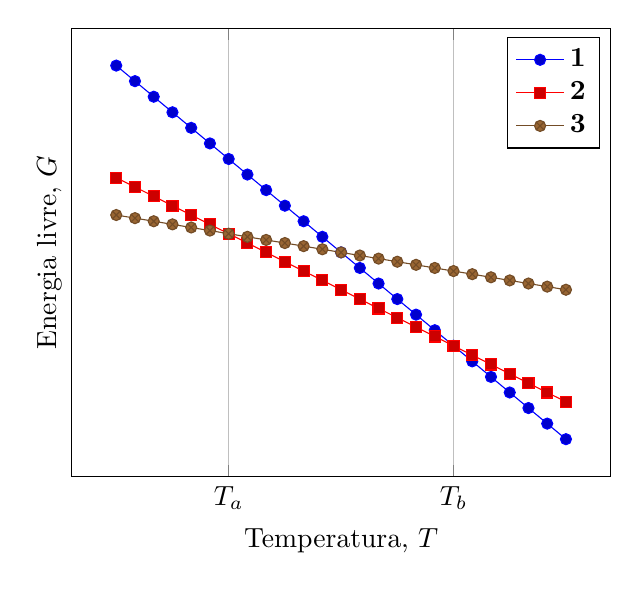
\begin{tikzpicture}
    \begin{axis}
        [
            grid = major,
            ylabel = {Energia livre, $G$},
            xlabel = {Temperatura, $T$},
            domain = -0.5:5.5,
            xtick= {1, 4}, 
            xticklabels={$T_a$, $T_b$},
            ytick=\empty,
        ]
        \addplot
            {
               11-5*x
            };
        \addplot
            {
               3-3*x
            };
        \addplot
            {
               1-x
            };
        \legend{{\textbf{1}},{\textbf{2}},{\textbf{3}}}
\end{axis}
\end{tikzpicture}